\documentclass[12pt]{article}
\usepackage{url,amsmath,setspace,amssymb,amsthm,amsfonts}


\setlength{\oddsidemargin}{.25in}
\setlength{\evensidemargin}{.25in}
\setlength{\textwidth}{6.25in}
\setlength{\topmargin}{-0.4in}
\setlength{\textheight}{8.5in}

\newcommand{\heading}[5]{
   \renewcommand{\thepage}{#1-\arabic{page}}
   \noindent
   \begin{center}
   \framebox[\textwidth]{
     \begin{minipage}{0.9\textwidth} \onehalfspacing
       {\bf CS 290G -- Introduction to Modern Cryptography} \hfill #2

       {\centering \Large #5
       
       }\medskip

       {\it #3 \hfill #4}
     \end{minipage}
   }
   \end{center}
}

\newcommand{\handout}[3]{\heading{#1}{#2}{Instructor:
Stefano Tessaro}{Scribe: Shiyu Ji}{Lecture #1: #3}}

\setlength{\parindent}{0in}

\newcommand{\eqdef}{\stackrel{def}{=}}
\newcommand{\N}{\mathbb{N}}
\newcommand{\R}{\mathbb{R}}
\newcommand{\Z}{\mathbb{Z}}
\newcommand{\F}{\mathbb{F}}
\newcommand{\bits}{\{0,1\}}
\newcommand{\inr}{\in_{\mbox{\tiny R}}}
%\newcommand{\getsr}{\gets_{\mbox{\tiny R}}}
\newcommand{\getsr}{\stackrel{\$}{\gets}}
\newcommand{\st}{\mbox{ s.t. }}
\newcommand{\etal}{{\it et al }}
\newcommand{\into}{\rightarrow}

\newcommand{\Ex}{\mathbb{E}}
\newcommand{\e}{\epsilon}
\newcommand{\ee}{\varepsilon}
\newcommand{\ceil}[1]{{\lceil{#1}\rceil}}
\newcommand{\floor}[1]{{\lfloor{#1}\rfloor}}
\newcommand{\angles}[1]{\langle #1 \rangle}
\newcommand{\Com}{{\sf Com}}
\newcommand{\desc}{{\sf desc}}

\newcommand{\rightstep}[1]{%
$\underrightarrow{\quad #1 \quad}$ }

\newcommand{\leftstep}[1]{%
$\underleftarrow{\quad #1 \quad}$ }

\newcommand{\Adv}{\mathsf{Adv}}

\newcommand{\tab}{\hspace{0.3in}}
%%%%%%%%%%%%%%%%%%%%%%%%%%%%
% Theorems & Definitions


\newtheorem{theorem}{Theorem}[section]

\newtheorem{claim}[theorem]{Claim}
\newtheorem{subclaim}{Claim}[theorem]
\newtheorem{proposition}[theorem]{Proposition}
\newtheorem{lemma}[theorem]{Lemma}
\newtheorem{corollary}[theorem]{Corollary}
\newtheorem{conjecture}[theorem]{Conjecture}

\theoremstyle{definition}
\newtheorem{definition}[theorem]{Definition}
\newtheorem{construction}[theorem]{Construction}
\newtheorem{example}[theorem]{Example}
\newtheorem{algorithm1}[theorem]{Algorithm}
\newtheorem{protocol}[theorem]{Protocol}
\newtheorem{remark}[theorem]{Remark}
\newtheorem{observation}[theorem]{Observation}
\newtheorem{assumption}[theorem]{Assumption}
\newtheorem{fact}[theorem]{Fact}

%\bibliographystyle{plain}
\usepackage{tikz}
\usetikzlibrary{calc,decorations.pathreplacing}

\begin{document}
\handout{5}{Jan 21, 2016}{Pseudorandom Functions}
\section{Recap}
Last lecture we constructed a PRG with extended outputs. That is, given a PRG $G : \bits^\lambda \mapsto \bits^{\lambda+k}$, we built another generator $G_t : \bits^\lambda \mapsto \bits^{\lambda+tk}$, and we also proved that if $G$ is a PRG and $t$ is polynomial in $\lambda$, then $G_t$ is also a PRG. The proof idea is to show that for all PPT distinguisher $D$, there exists a PPT distinguisher $D^*$ s.t.
$$\Adv_{G_t,\lambda}^{prg}(D) = t\cdot \Adv_{G,\lambda}^{prg}(D^*).$$
We ``fix'' some $D$, which expects input of $\lambda+kt$ bits, and construct $D^*$ based on the fixed $D$. $D^*$ expects $\lambda+k$ bits of input.
\begin{quote}
Distinguisher $D^* (y)$: here $y\in\bits^{\lambda+k}$ (it can be $y = G(s)$, $s\getsr\bits^\lambda$ or $y\getsr\bits^{\lambda+k}$)
\begin{enumerate}
\item $i \getsr \{1,2,\cdots,t\}$.
\item {\bf run} $D_i^* (y)$ and {\bf return} its output.
\end{enumerate}
\end{quote}
Each procedure $D_i^*(y)$ runs $D$ on $(z_1,z_2,\cdots,z_t,s_t)$, where $z_1,z_2,\cdots,z_{i-1}$ are uniformly random, $(s_i, z_i)$ is given by $y$, and $z_{i+1}, \cdots, z_t, s_t$ are generated by $G$ in the following way: 
$$(s_i,z_i)\gets y,$$
$$(s_{j+1}, z_{j+1}) \gets G(s_j, z_j),$$
for all $j$ s.t. $i\leq j < t$.
At the end, $D_i^*$ outputs the output of $D$.

Our goal is to calculate the advantage $\Adv_{G,\lambda}^{prg}(D^*)$. Before that we make a few observations on the output distribution of $D_i^*$. 

Denote by $H_i(y)$ the distribution of $(z_1,z_2,\cdots,z_t,s_t)$ given to $D$ in $D_i^*(y)$.
\begin{observation}
$$\Pr [s \getsr \bits^\lambda : D_1^*(G(s))=1] = \Pr[s \getsr \bits^\lambda : D(G_t(s))=1],$$
since in $D_1^*(G(s))$ every $z_i$ is produced by $G$, i.e., $H_1(G(s))=H_0(s)$ is the distribution of $G_t(s)$ given $s\getsr\bits^\lambda$.
\end{observation}

\begin{observation}
$$\Pr [y \getsr \bits^{\lambda+k} : D_t^*(y)=1] = \Pr [(z_1, z_2, \cdots, z_t, s_t) \getsr \bits^{\lambda+tk} : D(z_1, z_2, \cdots, z_t, s_t)=1],$$
since in $D_t^*$ every $z_t$ is at uniformly random, i.e., $H_t(y) = U_{\lambda+tk}$ given $y \getsr \bits^{\lambda+k}$.
\end{observation}

\begin{observation}
For any $i\in\{1,2,\cdots,t-1\}$,
$$\Pr [y \getsr \bits^{\lambda+k} : D_i^*(y)=1] = \Pr [s \getsr \bits^\lambda : D_{i+1}^*(G(s))=1].$$
Figure \ref{fig:2h} gives the reason.
\end{observation}

\begin{figure}[!t]
\centering{}
\begin{tikzpicture}
% s_i
\node at (1.3,1) {$\cdots$};
\draw (4,0) rectangle (5,2); \node at (4.5, 1) {$s_i$};
\draw (6,0) rectangle (7,2); \node at (6.5, 1) {$s_{i+1}$};
\draw (10,0) rectangle (11,2); \node at (10.5, 1) {$s_{t-1}$};
\draw (12,0) [fill = lightgray] rectangle (13,2); \node at (12.5, 1) {$s_t$};
% z_i
\draw [fill = lightgray] (-2,2) rectangle (-1,3); \node at (-1.5, 2.5) {$z_1$}; 
\draw [fill = lightgray] (-0.5,2) rectangle (0.5,3); \node at (0, 2.5) {$z_2$};
\draw [fill = lightgray] (2,2) rectangle (3,3); \node at (2.5, 2.5) {$z_{i-1}$};
\draw [fill = lightgray] (4,2) rectangle (5,3); \node at (4.5, 2.5) {$z_i$};
\draw [fill = lightgray] (6,2) rectangle (7,3); \node at (6.5, 2.5) {$z_{i+1}$};
\draw [fill = lightgray] (10,2) rectangle (11,3); \node at (10.5, 2.5) {$z_{t-1}$};
\draw [fill = lightgray] (12,2) rectangle (13,3); \node at (12.5, 2.5) {$z_t$};
% arrows
\draw [->, thick] (5,1) -- (6,1); \node [above] at (5.5,1) {$G$};
\draw [->, thick] (7,1) -- (8,1); \node [above] at (7.5,1) {$G$};
\node at (8.5,1) {$\cdots$};
\draw [->, thick] (9,1) -- (10,1); \node [above] at (9.5,1) {$G$};
\draw [->, thick] (11,1) -- (12,1); \node [above] at (11.5,1) {$G$};
% misc
\draw [decorate,decoration={brace, amplitude=7pt}] (4,0) -- (4,2);
\node [left] at (3.8,1) {$\lambda$};
\draw [decorate,decoration={brace, amplitude=7pt}] (0.5,3) -- (0.5,2);
\node [right] at (0.7,2.5) {$k$};
\node at (-.5,1) {$H_i(U_{\lambda+k})$};
\node at (2,.3) {$(s_i,z_i)\gets y$};
\end{tikzpicture}

\vspace{.2in}

\begin{tikzpicture}
% s_i
\node at (1.3,1) {$\cdots$};
\draw (4,0) rectangle (5,2); \node at (4.5, 1) {$s$};
\draw (6,0) rectangle (7,2); \node at (6.5, 1) {$s_{i+1}$};
\draw (10,0) rectangle (11,2); \node at (10.5, 1) {$s_{t-1}$};
\draw (12,0) [fill = lightgray] rectangle (13,2); \node at (12.5, 1) {$s_t$};
% z_i
\draw [fill = lightgray] (-2,2) rectangle (-1,3); \node at (-1.5, 2.5) {$z_1$}; 
\draw [fill = lightgray] (-0.5,2) rectangle (0.5,3); \node at (0, 2.5) {$z_2$};
\draw [fill = lightgray] (2,2) rectangle (3,3); \node at (2.5, 2.5) {$z_{i-1}$};
\draw [fill = lightgray] (4,2) rectangle (5,3); \node at (4.5, 2.5) {$z_i$};
\draw [fill = lightgray] (6,2) rectangle (7,3); \node at (6.5, 2.5) {$z_{i+1}$};
\draw [fill = lightgray] (10,2) rectangle (11,3); \node at (10.5, 2.5) {$z_{t-1}$};
\draw [fill = lightgray] (12,2) rectangle (13,3); \node at (12.5, 2.5) {$z_t$};
% arrows
\draw [->, thick] (5,1) -- (6,1); \node [above] at (5.5,1) {$G$};
\draw [->, thick] (7,1) -- (8,1); \node [above] at (7.5,1) {$G$};
\node at (8.5,1) {$\cdots$};
\draw [->, thick] (9,1) -- (10,1); \node [above] at (9.5,1) {$G$};
\draw [->, thick] (11,1) -- (12,1); \node [above] at (11.5,1) {$G$};
% misc
\draw [decorate,decoration={brace, amplitude=7pt}] (4,0) -- (4,2);
\node [left] at (3.8,1) {$\lambda$};
\draw [decorate,decoration={brace, amplitude=7pt}] (0.5,3) -- (0.5,2);
\node [right] at (0.7,2.5) {$k$};
\node at (-.5,1) {$H_{i+1}(G(U_\lambda))$};
\end{tikzpicture}
\caption{The distributions $H_i(U_{\lambda+k})$ and $H_{i+1}(G(U_\lambda))$. It turns out that they are the same distribution, since $y\getsr\bits^{\lambda+k}$ and $s\getsr\bits^{\lambda}$.}
\label{fig:2h}
\end{figure}

Based on these observations, we can compute the advantage:
$$
\begin{aligned}
&\Adv_{G,\lambda}^{prg}(D^*) \\
=& \bigg| \Pr[s \getsr \bits^\lambda : D^*(G(s)) = 1] - \Pr[y \getsr \bits^{\lambda+k} : D^*(y) = 1] \bigg| \\
=& \bigg| \frac{1}{t}\sum_{i=1}^t \Pr[s \getsr \bits^\lambda : D_i^*(G(s)) = 1] - \frac{1}{t}\sum_{i=1}^t \Pr[y \getsr \bits^{\lambda+k} : D_i^*(y) = 1] \bigg| \\
=& \frac{1}{t}\bigg| \sum_{i=1}^t \Pr[s \getsr \bits^\lambda : D_i^*(G(s)) = 1] - \sum_{i=1}^t \Pr[y \getsr \bits^{\lambda+k} : D_i^*(y) = 1] \bigg| \\
=& \frac{1}{t}|p_1 - q_t| = \frac{1}{t} \Adv_{G_t, \lambda}^{prg}(D).
\end{aligned}
$$
Note that our observations can cancel out $t-2$ terms.

Last lecture we also saw a concrete construction of PRG given by Blum and Micali \cite{BM84}.
Given a large prime modulus $p$, and a generator $g$ of $\Z_p^*$, the seed is $s \in \Z_p^* = \{1,2,\cdots,p-1\}$, and we build a generator $BM_t : \Z_p^* \mapsto \bits^t$ as following.
\begin{quote}
Procedure $BM_t(s)$: ($t$ is roughly larger than $\log p$)
\begin{enumerate}
\item $s_0 \gets s$.
\item {\bf for} $i=1$ to $t$ {\bf do}
\item \tab $s_i \gets g^{s_{i-1}} \mod p$.
\item \tab $z_i \gets MSB(s_i)$.
\item {\bf return} $z_1,z_2,\cdots,z_t$.
\end{enumerate}
\end{quote}
The most significant bit (MSB) is defined as:
$$MSB(x) \eqdef \begin{cases}
1, & \textrm{if } x>\frac{p-1}{2}, \\
0, & \textrm{otherwise.}
\end{cases}.$$
We can show that Blum-Micali's construction is a PRG assuming discrete logarithm problem (DLP) is hard.
\begin{theorem}
If DLP is hard to solve, then $BM_t$ is a PRG.
\end{theorem}

\section{Pseudorandom Functions}
Given $\lambda$ bits of input, a PRG can output at most poly($\lambda$) pseudorandom bits. 
However, this is not always what we want.
The question is: is it possible to build an efficient generator that can output $2^\lambda$ of pseudorandom bits given $\lambda$ input bits?
The answer is no, because it requires at least $2^\lambda$ time and thus is not efficient. This motivates our second-best goal: given $s\in\bits^\lambda$ and an index $i\in\{1,2,3,\cdots,2^\lambda\}$, can we efficiently compute the individual bits of $G(s)$?
It turns out this goal can be achieved, and it gives rise to pseudorandom functions (PRFs).

We start from a simple example. Assume we have a doubling PRG $G : \bits^\lambda \mapsto \bits^{2\lambda}$. The goal is to build a PRG $G' : \bits^\lambda \mapsto \bits^{4\lambda}$. Rather than calculating the bits sequentially as before, we can do it in a more parallel mode (Figure \ref{fig:2tree}). 

\begin{figure}[!t]
\centering{}
\begin{tikzpicture}
\draw (4,4) rectangle (6,5); \node at (5,4.5) {$s$};
\draw [->, thick] (5,4) -- (5,3); \node [left] at (5,3.5) {$G$};
\draw (3,2) rectangle (5,3); \node at (4,2.5) {$s_0$};
\draw [->, thick] (4,2) -- (4,1); \node [left] at (4,1.5) {$G$};
\draw (5,2) rectangle (7,3); \node at (6,2.5) {$s_1$};
\draw [->, thick] (6,2) -- (6,1); \node [right] at (6,1.5) {$G$};
\draw (0.5,0) rectangle (2.5,1); \node at (1.5,0.5) {$s_{00}$};
\draw (2.5,0) rectangle (4.5,1); \node at (3.5,0.5) {$s_{01}$};
\draw (5.5,0) rectangle (7.5,1); \node at (6.5,0.5) {$s_{10}$};
\draw (7.5,0) rectangle (9.5,1); \node at (8.5,0.5) {$s_{11}$};
\end{tikzpicture}
\caption{A PRG $G' : \bits^\lambda \mapsto \bits^{4\lambda}$ based on PRG $G : \bits^\lambda \mapsto \bits^{2\lambda}$.}
\label{fig:2tree}
\end{figure}

We can easily extend this tree-like construction to the case of $\bits^\lambda \mapsto \bits^{2^n\cdot\lambda}$ (Figure \ref{fig:ntree}).
If we want to get any bits at the $2^n$ $\lambda$-bit blocks, we can make $n$ calls to $G$ along the path by index.

\begin{figure}[!t]
\centering{}
\begin{tikzpicture}
\draw (4,4) rectangle (6,5); \node at (5,4.5) {$s$};
\draw [->, thick] (5,4) -- (5,3); \node [left] at (5,3.5) {$G$};
\draw (3,2) rectangle (5,3); \node at (4,2.5) {$s_0$};
\draw [->, thick] (4,2) -- (4,1); \node [left] at (4,1.5) {$G$};
\draw (5,2) rectangle (7,3); \node at (6,2.5) {$s_1$};
\draw [->, thick] (6,2) -- (6,1); \node [right] at (6,1.5) {$G$};
\draw (0.5,0) rectangle (2.5,1); \node at (1.5,0.5) {$s_{00}$};
\draw [->, thick] (1.5,0) -- (1.5,-1); \node [right] at (1.5,-0.5) {$G$}; \node at (1.5,-1.5) {$\cdots$};
\draw (2.5,0) rectangle (4.5,1); \node at (3.5,0.5) {$s_{01}$};
\draw [->, thick] (3.5,0) -- (3.5,-1); \node [right] at (3.5,-0.5) {$G$}; \node at (3.5,-1.5) {$\cdots$};
\draw (5.5,0) rectangle (7.5,1); \node at (6.5,0.5) {$s_{10}$};
\draw [->, thick] (6.5,0) -- (6.5,-1); \node [right] at (6.5,-0.5) {$G$}; \node at (6.5,-1.5) {$\cdots$};
\draw (7.5,0) rectangle (9.5,1); \node at (8.5,0.5) {$s_{11}$};
\draw [->, thick] (8.5,0) -- (8.5,-1); \node [right] at (8.5,-0.5) {$G$}; \node at (8.5,-1.5) {$\cdots$};
\draw (0,-3) rectangle (2,-2); \draw (2,-3) rectangle (4,-2);
\node at (1,-2.5) {$s_{000\cdots 00}$}; \node at (3,-2.5) {$s_{000\cdots 01}$};
\node at (5,-2.5) {$\cdots$};
\draw (6,-3) rectangle (8,-2); \draw (8,-3) rectangle (10,-2);
\node at (7,-2.5) {$s_{111\cdots 10}$}; \node at (9,-2.5) {$s_{111\cdots 11}$};
\node at (12, 4.5) {$1$};
\node at (12, 2.5) {$2$};
\node at (12, 0.5) {$2^2$};
\node at (12, -2.5) {$2^n$};
\end{tikzpicture}
\caption{A PRG $G' : \bits^\lambda \mapsto \bits^{2^n\cdot\lambda}$ based on PRG $G : \bits^\lambda \mapsto \bits^{2\lambda}$.}
\label{fig:ntree}
\end{figure}

Based on this idea, Goldreich, Goldwasser and Micali \cite{GGM86} gave the construction $GGM : \bits^\lambda \times \bits^n \mapsto \bits^\lambda$ as following:
\begin{quote}
Procedure $GGM(s,x)$: ($x=x_1x_2\cdots x_n$)
\begin{enumerate}
\item $s_0 \gets s$.
\item {\bf for} $i=1$ to $n$ {\bf do}
\item \tab $(y_0, y_1) \gets G(s_{i-1})$.
\item \tab $s_i \gets y_{x_i}$.
\item {\bf return} $s_n$.
\end{enumerate}
\end{quote}
It turns out $GGM$ is a PRF, which should behave like a ``random function'' (RF). We need to formally define what RF is.
\begin{definition}
$RF_{n,m}$ is a ``system'' that takes inputs from $\bits^n$ and produces outputs from $\bits^m$. Its behaviors are given below:

We use a table $T$ to keep the states, i.e., for any $x\in\bits^n$, $T[x] \in \bits^m \cup \{\bot\}$, where $\bot$ is a special symbol meaning $T[x]$ is not set. Initially, $T[x] = \bot$ for any $x\in\bits^n$. Then upon input $x$, $RF_{n,m}(x)$ is defined as:
\begin{quote}
Procedure $RF_{n,m}(x)$:
\begin{enumerate}
\item {\bf if} $T[x] = \bot$ {\bf then}
\item \tab $T[x] \getsr \bits^m$.
\item {\bf return} $T[x]$.
\end{enumerate}
\end{quote}
\end{definition}
Informally, random function $RF_{n,m}$ is a box answering queries $x_1,x_2,\cdots$ by returning the query results $y_1,y_2,\cdots$. The query results should be consistent, i.e., $x_i = x_j$ implies $y_i = y_j$. The table $T$ can guarantee the consistence.

Now we can give the formal definition of PRF.
\begin{definition}
A function $F : \bits^\lambda \times \bits^{n(\lambda)} \mapsto \bits^{m(\lambda)}$ is a PRF if
\begin{enumerate}
\item It is efficiently computable.
\item For any PPT distinguisher $D$,
$$\Adv_{F,\lambda}^{prf}(D) \eqdef \bigg| \Pr[s \getsr \bits^\lambda: D^{F(s,\cdot)}=1] - \Pr[D^{RF_{n,m}}=1] \bigg|$$
is negligible. Here $D^{O}$ means that $D$ can make queries to $O$, which is a black box (aka oracle) that answers each query. 
\end{enumerate}
\end{definition}

The definition of PRF can be illustrated by a random experiment (Figure \ref{fig:re}).

\begin{figure}[!t]
\centering{}
\begin{tikzpicture}
\draw (1,0) rectangle (3,1); \node at (2,0.5) {$D$}; \draw [->] (1,0.5) -- (0,0.5); \node [above] at (0.5,0.5) {$0/1$};
\draw (5,0) rectangle (7,1); \node at (6,0.5) {$F(s,\cdot)$}; 
\draw [->] (3,0.6) -- (5,0.6); \node [above] at (4,0.6) {\scriptsize $x_i\in\bits^n$};
\draw [->] (5,0.4) -- (3,0.4); \node [below] at (4,0.4) {\scriptsize $y_i = F(s,x_i)$};

\draw [dashed, thick] (7.5,0) -- (7.5,1);

\draw (9,0) rectangle (11,1); \node at (10,0.5) {$D$};  \draw [->] (9,0.5) -- (8,0.5); \node [above] at (8.5,0.5) {$0/1$};
\draw (13,0) rectangle (15,1); \node at (14,0.5) {$RF_{n,m}$}; 
\draw [->] (11,0.6) -- (13,0.6); \node [above] at (12,0.6) {$x_i$};
\draw [->] (13,0.4) -- (11,0.4); \node [below] at (12,0.4) {$y_i$};
\end{tikzpicture}
\caption{Random experiment between the distinguisher $D$ and a black box, which can be either $RF_{n,m}$ or $F(s,\cdot)$ given $s\getsr\bits^\lambda$.}
\label{fig:re}
\end{figure}

We give an example which is \emph{not} a PRF.
\begin{example}
A function $F : \bits^\lambda \times \bits^\lambda \mapsto \bits^{\lambda}$ s.t. $F(s,x) = s \oplus x$.

To show $F$ is not a PRF, we need to find a distinguisher $D$ s.t. $\Adv_{F,\lambda}^{prf}(D)$ is non-negligible.
\begin{quote}
Distinguisher $D^O$:
\begin{enumerate}
\item $s' \gets O(0^\lambda)$.
\item $y \gets O(s')$.
\item {\bf if} $y=0^\lambda$ {\bf then return} 1.
\item {\bf else return} 0.
\end{enumerate}
\end{quote}
Here $O(q)$ denotes the answer given by the black box $O$ to the query $q$ from $D$.

It is straightforward to see $\Pr[D^{F(s,\cdot)}=1]=1$ and $\Pr[D^{RF_{n,m}}=1]=2^{-\lambda}$. Thus $\Adv_{F,\lambda}^{prf}(D)=1-2^{-\lambda}$, which is overwhelming.
\end{example}

In fact, $GGM$ is a PRF construction based on PRG $G$.
\begin{theorem}
If $G$ is a PRG, then $GGM$ is a PRF.
\end{theorem}

\begin{thebibliography}{10}

\bibitem{BM84}
M. Blum and S. Micali, 1984. 
How to generate cryptographically strong sequences of pseudorandom bits. 
SIAM journal on Computing, 13(4), pp. 850-864.

\bibitem{GGM86}
O. Goldreich, S. Goldwasser. and S. Micali, 1986. 
How to construct random functions. 
Journal of the ACM (JACM), 33(4), pp.792-807.

\end{thebibliography}

\end{document}
